% -*- TeX-master: "main"; fill-column: 72 -*-
\section{Package syntax and semantics}

In this section, we define the syntax and semantics of the
\RenderPackage for \sbmlthreecore. We expound on the various data types
and constructs defined in this package, then in \sec{examples}, we
provide complete examples of using the constructs in example SBML
models.

%----------------------------------------
%----------------------------------------
\subsection{Namespace URI and other declarations necessary for using
this package}
\label{xml-namespace}

Every SBML Level~3 package is identified uniquely by an XML namespace
URI. For an SBML document to be able to use a given SBML Level~3
package, it must declare the use of that package by referencing its URI.
The following is the namespace URI for this version of the
\RenderPackage for SBML Level~3 Version~1:

\begin{center}
\uri{http://www.sbml.org/sbml/level3/version1/render/version1}
\end{center}

In addition, SBML documents using a given package must indicate whether
understanding the package is required for complete mathematical
interpretation of a model, or whether the package is optional. This is
done using the attribute \token{required} on the \token{<sbml>} element
in the SBML document. For the \RenderPackage the value of the required
attribute is \val{false}.

The following fragment illustrates the beginning of a typical SBML model
using SBML Level~3 Version~1 and this version of the \RenderPackage (note, that the Layout package is also needed):

\begin{example}
<?xml version="1.0" encoding="UTF-8"?>
 <sbml xmlns="http://www.sbml.org/sbml/level3/version1/core" level="3" version="1"
   xmlns:layout="http://www.sbml.org/sbml/level3/version1/layout/version1" layout:required="false"
   xmlns:render="http://www.sbml.org/sbml/level3/version1/render/version1" render:required="false"
	>
	
\end{example}


Originally the layout and render extension were developed for use with SBML Level 2 files, where the information was stored in annotations to SBML models, layout lists and layouts.
The namespace for the version of the SBML render extension for SBML level 2 is: 

\begin{center}
\uri{http://projects.eml.org/bcb/sbml/render/level2}
\end{center}

An example using the render extension in this context would look like this: 

\begin{example}
<?xml version="1.0" encoding="utf-8"?>
<sbml xmlns="http://www.sbml.org/sbml/level2" level="2" version="1">
  <model id="model1" name="Model with L2 Render Annotation">
    <annotation>
      <listOfLayouts xmlns="http://projects.eml.org/bcb/sbml/level2">
        <layout id="layout1">
          <annotation>
            <listOfRenderInformation xmlns="http://projects.eml.org/bcb/sbml/render/level2">
							...
            </listOfRenderInformation>
          </annotation>
					...
        </layout>
				...
      </listOfLayouts>
			...
    </annotation>
		...
  </model>
</sbml>
\end{example}

%--------------------------------------------------
\subsection{Primitive data types}
\label{primitive-types}

Section~3.1 of the SBML Level~3 specification defines a number of
primitive data types and also uses a number of XML Schema 1.0 data types
\citep{biron:2000}. We assume and use some of them in the rest of this
specification, specifically \primtype{boolean}, \primtype{integer}, \primtype{double}, \primtype{ID},
\primtype{SId}, \primtype{SIdRef}, and \primtype{string}. The
\RenderPackage defines other primitive types; these are described below.

%\TODO{check all necessary types from core are listed}

%-----------------------------------------------
\subsubsection{Type \fixttspace\primtypeNC{StyleType}}

The type \primtype{StyleType} is used by \LocalStyle and \GlobalStyle elements, in order
to apply a particular \Style to a \GraphicalObject. This is done via the \token{typeList} attribute
that uses the \primtype{StyleType} as its data type. 

A valid \StyleType instance is a combination of one or more of the following 
values separated by white spaces:

\begin{itemize}
 \item \val{COMPARTMENT\-GLYPH},
 \item \val{SPECIES\-GLYPH},
 \item \val{REACTION\-GLYPH}, 
 \item \val{SPECIES\-REFERENCE\-GLYPH},
 \item \val{TEXT\-GLYPH}, 
 \item \val{GENERAL\-GLYPH}, 
 \item \val{GRAPHICAL\-OBJECT} 
 \item \val{ANY}
\end{itemize}

The \token{ANY} keyword specifies that this styles applies to any type of glyph and 
would be equivalent to listing all the other keywords. 

%-----------------------------------------------
\subsubsection{Type \fixttspace\primtypeNC{GradientSpreadMethod}}

The type \GradientSpreadMethod is being used by \GradientBase elements to decide how 
gradients propagate over the whole element they are applied to. It is an enumeration consisting 
of the following three values called \texttt{pad}, \texttt{reflect} or \texttt{repeat}:

\begin{itemize}
 \item {\texttt{pad}:} the gradient color at the
endpoint of the vector defines how the gradient is continued beyond that point (default value).
 \item {\texttt{reflect}:} the gradient continues from end to start and
then from start to end again and again.
 \item {\texttt{repeat}:} the gradient pattern is repeated from start to end over and over again.
\end{itemize}

\begin{figure}[!ht]
\begin{center}
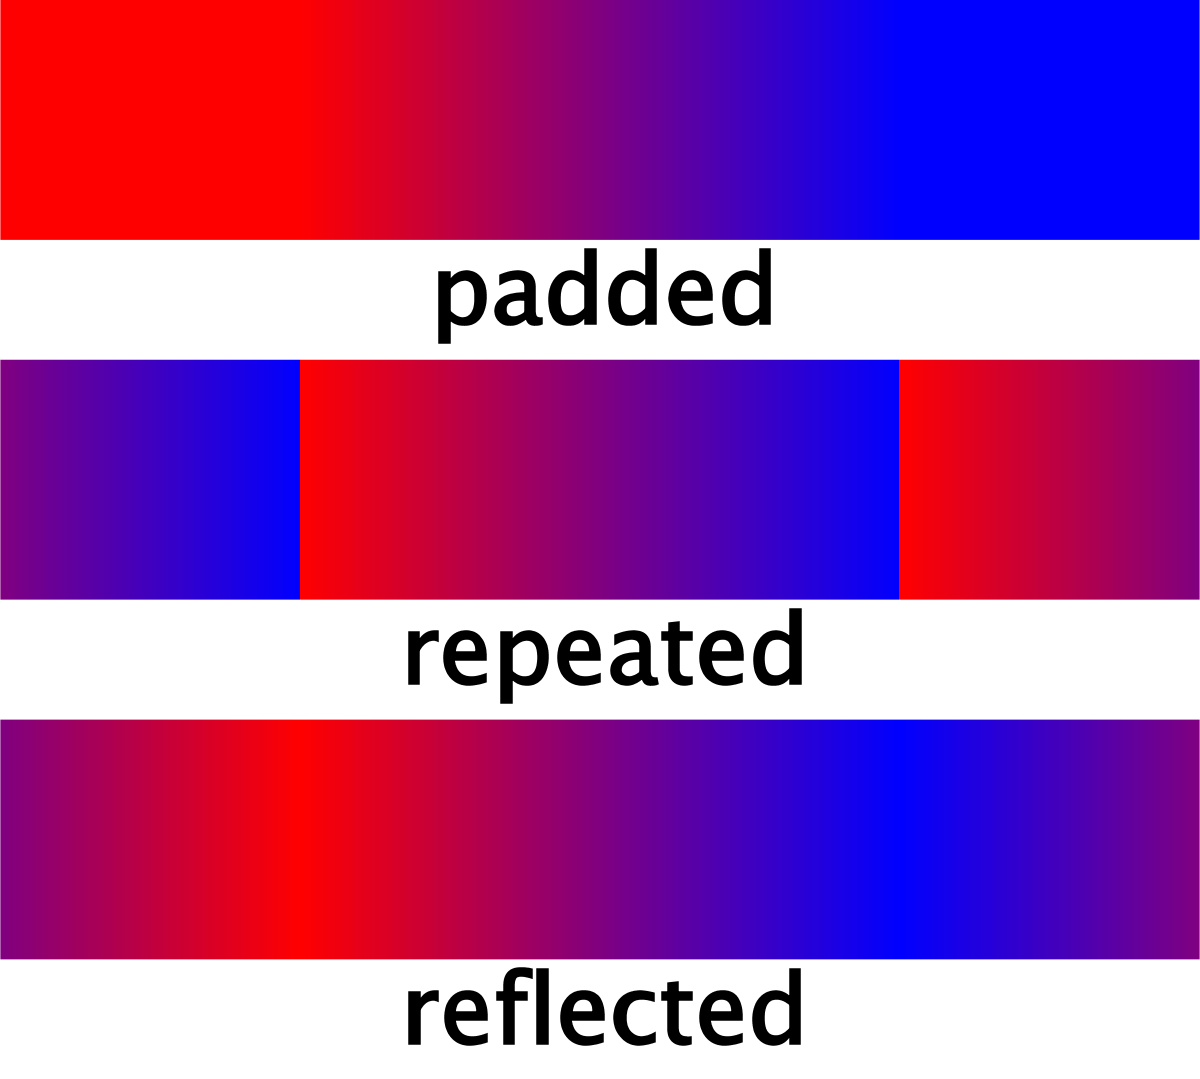
\includegraphics[scale=0.18]{figures/SVG_spreadMethod.png}
\end{center}
\caption{example of different SVG spreadMethod values}
\label{SVG:spreadMethod}
\end{figure}

%-----------------------------------------------
\subsubsection{Type \fixttspace\primtypeNC{FillRule}}

The type FillRule describes how a surface created by connecting 
points on a \Polygon are to be filled when rendered. Allowed values for a valid instance of type \primtype{FillRule} are:

\begin{itemize}
 \item \token{nonzero} 
 \item \token{evenodd}
\end{itemize}

For a detailed description on how those attributes work in detail, we would like to refer you to the corresponding documentation in the \needref{SVG specification}. 
\TODO{which attributes does this sentence mean}

%-----------------------------------------------
\subsubsection{Type \fixttspace\primtypeNC{FontFamily}}

The \FontFamily type gives a hint as to which font is to be used when
rendering \Text elements. This type extends the type \primtype{string}. The following values are pre-defined: 

\begin{itemize}
 \item \token{serif},
 \item \token{sans-serif}
 \item \token{monospace}
\end{itemize}

However, applications are free to use the \FontFamily to store the name of the font the writing application used as a string. It has not been a issue for reading applications to find a similar font. 

%-----------------------------------------------
\subsubsection{Type \fixttspace\primtypeNC{FontWeight}}
The type \FontWeight indicates whether the font is to be used in its normal form, or in its bold form. Consequently, the only values allowed for this enumeration are: 

\begin{itemize}
 \item \token{bold} 
 \item \token{normal} 
\end{itemize}

%-----------------------------------------------
\subsubsection{Type \fixttspace\primtypeNC{FontStyle}}

The type \FontStyle determines whether a font is to be
drawn use italic or normal styles. Thus the only allowed values are:

\begin{itemize}
 \item \token{italic} 
 \item \token{normal} 
\end{itemize}

%-----------------------------------------------
\subsubsection{Type \fixttspace\primtypeNC{VTextAnchor}}

The type VTextAnchor allows models to specify how text elements are to be
vertically aligned within their bounding box. This enumeration has the following allowed values: 

\begin{itemize}
 \item \token{top},
 \item \token{middle},
 \item \token{bottom} 
 \item \token{baseline}
\end{itemize}

Examples illustration the use of the different \VTextAnchor values are given in Appendix \ref{apdx-text-anchor}.




%-----------------------------------------------
\subsubsection{Type \fixttspace\primtypeNC{HTextAnchor}}

The type \HTextAnchor defines the horizontal alignment of text elements. This enumeration can use the following values: 

\begin{itemize}
 \item \token{start},
 \item \token{middle}
 \item \token{end}
\end{itemize}

Examples illustration the use of the different \HTextAnchor values are given in Appendix \ref{apdx-text-anchor}.



%-----------------------------------------------
\subsubsection{Type \fixttspace\primtypeNC{RelAbsVector}}

The position and size of render elements can be specified as a combination of an absolute value and a relative value. The absolute value is a numerical value in units of \val{pt} (1/72 inch) indicating the position of the object. The relative value is a percentage indicating the size of the object. All values are relative to the bounding box of the corresponding element in the layout. This bounding box basically specifies a canvas for the render elements to be drawn on.

In order to avoid populating the resulting XML with numerous attributes the \RenderPackage encodes this information in the \RelAbsVector class with the two attributes \token{abs} and \token{rel} by extending the \primtype{string} such that it encodes optionally an absolute number first followed by an optional 
relative number followed by a \% sign. 

Examples of the \RelAbsVector construct are shown in the table below.
\smallskip
\begin{center}
\begin{tabular}{ | l | p{5cm} |}
\hline
\primtype{string} & Coordinate \\ \hline
$-5+100\%$ & 5 points left of the right edge of the current view \\ \hline
$50\%$ & FILL IN \\ \hline
$2$ & FILL IN \\ 
\hline
\end{tabular}
\end{center}
\smallskip
\TODO{Should there be a space between abs and rel value if both are used}

It should be noted that when applying transformations to elements with relative values, the relative 
values have to be converted to absolute values first.

%---------------------------------------------------------
%---------------------------------------------------------
\subsection{General features}

The render extension provides two locations where styles can be defined. First 
each layout can have its own set of render information located as a child element
of the \Layout element (\ref{fig:Render_uml}).  This is considered to be \textbf{local} render information.
Secondly, \textbf{global} render information objects can be located as child elements of the \ListOfLayouts element (\ref{fig:lol_render_uml}). 

\begin{figure}[h!]
  \centering
  % Requires \usepackage{graphicx}
  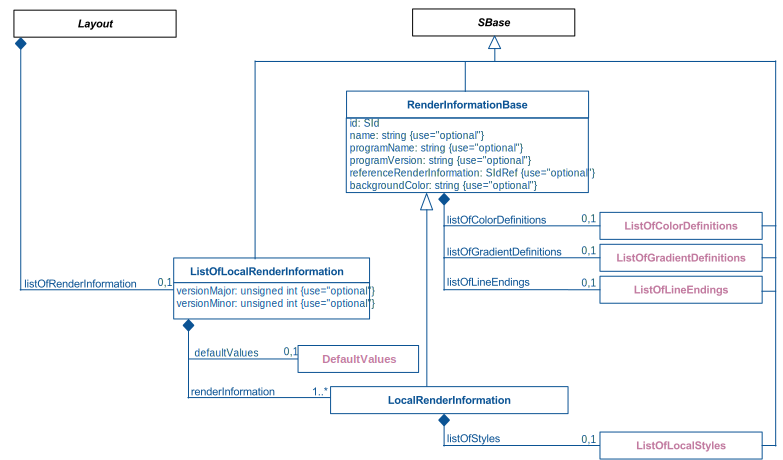
\includegraphics[width=\textwidth]{images/render-layout-uml}\\
  \caption{A UML representation of the extended \Layout class for the \RenderPackage. See \ref{conventions} for conventions related to this figure.}
  \label{fig:Render_uml}
\end{figure}

\begin{figure}[h!]
  \centering
  % Requires \usepackage{graphicx}
  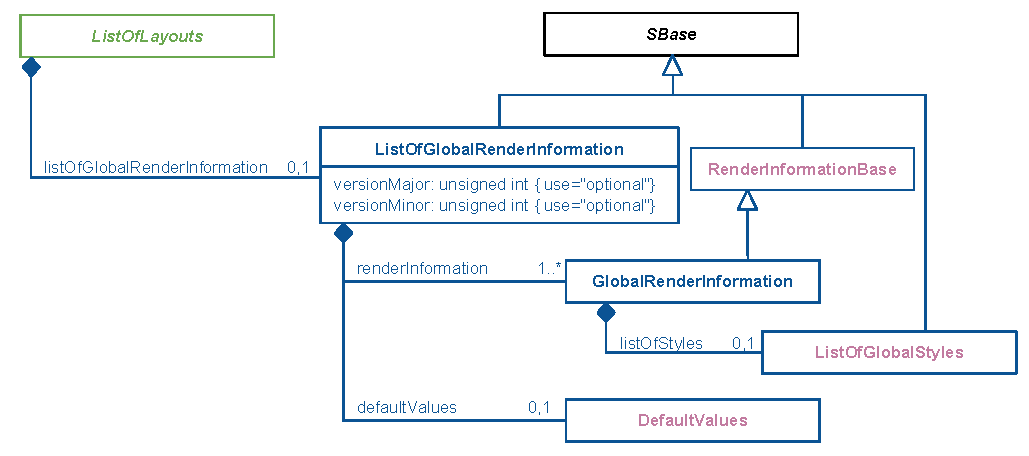
\includegraphics[width=\textwidth]{images/render-listoflayout-uml}\\
  \caption{A UML representation of the extended \ListOfLayouts object for the \RenderPackage.  See \ref{conventions} for conventions related to this figure. }
  \label{fig:lol_render_uml}
\end{figure}

It is important to note that each layout can have more than one 
set of local render information and that it is 
also possible to define more then one global style. Each style can also 
reference another style that complements it, this way the user can create 
styles that are based on other styles. In contrast to local styles, the global styles can not 
reference individual layout elements by an id, they can only define role based or 
type based styles.

%--------------------------------------------------------
\subsubsection{Uniqueness of ids}
Since local and global render information objects can reference other render information objects, programs creating
render information need to make sure that all the ids are unique within the reference history. In other words, a 
render information object that references another render information object must make sure that none of its ids is equal
to an id in any of the directly or indirectly referenced render information objects. 

An exception to this rule is that a \ColorDefinition may have the same \token{id} as a \ColorDefinition in a referenced style. In this case interpreting programs can assume that this \ColorDefinition is supposed to override the \ColorDefinition with the
same \token{id} in the referenced render information object. Likewise it is also possible to override a \ColorDefinition with a  gradient \need{does this mean either a \LinearGradient or a \RadialGradient or is it more open} and vice versa. \LineEnding definitions on the other hand can only be replaced by other \LineEnding definitions.

%----------------------------------------------------------
%----------------------------------------------------------
\subsection{Extended elements from the \LayoutPackage}


% ---------------------------------------------------------
\subsubsection{The extended \class{GraphicalObject} class}
\label{graphicalobject-class}

The \RenderPackage extends the \class{GraphicalObject} object from the \LayoutPackage with the
addition of
the \token{objectRole} attributes.

\paragraph{The \fixttspace\token{objectRole} attribute}


A \GraphicalObject has an optional attribute \token{objectRole} of type
\primtype{string}.  This attribute specifies with which \Style the object should be rendered.

\need{some sort of example here} 

% ---------------------------------------------------------
\subsubsection{The extended \class{ListOfLayouts} class}
\label{listoflayouts-class}

The \RenderPackage extends the \class{ListOfLayouts} object from the \LayoutPackage with the
addition of an optional \ListOfGlobalRenderInformation object (\ref{fig:lol_render_uml}).

% ---------------------------------------------------------
\paragraph{The \class{ListOfGlobalRenderInformation} class}
\label{listofglobalrenderinformation-class}

The \ListOfGlobalRenderInformation object derives from the
\class{ListOf} class and inherits the core attributes and subobjects from the
\class{SBase} class. It contains one or more objects of type
\GlobalRenderInformation.

In addition the \ListOfGlobalRenderInformation object has the required attributes \token{versionMajor} and \token{versionMinor}.

\paragraph{The \fixttspace\token{versionMajor} attribute}

A \ListOfGlobalRenderInformation has a required attribute
\token{versionMajor} of type \primtype{unsigned integer} which specifies the major version of the render information. Major versions do not have to be backwards compatible with any lower major version of the render specification.

\paragraph{The \fixttspace\token{versionMinor} attribute}

A \ListOfGlobalRenderInformation has a required attribute
\token{versionMinor} of type \primtype{unsigned integer} which specifies the minor version of the render information.  All minor versions within a major version have to be compatible.

\need{to explain how or indeed if these version numbers relate to sbml levels/versions}

% ---------------------------------------------------------
\subsubsection{The extended \class{Layout} class}
\label{layout-class}

The \RenderPackage extends the \class{Layout} object from the \LayoutPackage with the addition
of an optional  \ListOfLocalRenderInformation object (\ref{fig:Render_uml}).

% ---------------------------------------------------------
\paragraph{The \class{ListOfLocalRenderInformation} class}
\label{listoflocalrenderinformation-class}

The \ListOfLocalRenderInformation object derives from the \class{ListOf} class
and inherits the core attributes and subobjects from the \class{SBase}
class. It contains one or more objects of type \LocalRenderInformation.

In addition the \ListOfLocalRenderInformation object has the required \need{are these optional or required}
attributes \token{versionMajor} and \token{versionMinor}.

\paragraph{The \fixttspace\token{versionMajor} attribute}

A \ListOfLocalRenderInformation has a required attribute
\token{versionMajor} of type \primtype{unsigned integer} which specifies the major version of the render information. Major versions do not have to be backwards compatible with any lower major version of the render specification.

\paragraph{The \fixttspace\token{versionMinor} attribute}

A \ListOfLocalRenderInformation has a required attribute
\token{versionMinor} of type \primtype{unsigned integer} which specifies the minor version of the render information.  All minor versions within a major version have to be compatible.

\need{to explain how or indeed if these version numbers relate to sbml levels/versions}

%----------------------------------------------------------
%----------------------------------------------------------
\subsection{Render Information}
\label{renderinformation-class}
The render information classes hold all information about the rendering. The
information is stored between three classes: \RenderInformationBase, the base class with 
common features; \GlobalRenderInformation a class applying to types and roles of 
elements on a global level; and \LocalRenderInformation that provides additional information that can be applied to individual elements from the \LayoutPackage. These classes are illustrated in \ref{fig:Render_uml} and \ref{fig:lol_render_uml}.

% ---------------------------------------------------------
\subsubsection{The \class{RenderInformationBase} class}
\label{renderinformationbase-class}

The \RenderInformationBase class is an abstract class that holds all the information that is common to both local and global render 
information objects. It  derives from the \SBase class and thus
inherits any attributes and elements that are present on this class. In addition the \RenderInformationBase has the required attribute \token{id} and the 
optional attributes \token{name}, \token{programName}, \token{programVersion}, 
\token{referenceRenderInformation} and \token{backgroundColor}. Additionally it may
contain a \ListOfColorDefinitions, \ListOfGradientDefinitions and / or a \ListOfLineEndings.

\need{are the listOf optional or required}

\paragraph{The \fixttspace\token{id} attribute}

A \RenderInformationBase has a required attribute \token{id} of type
\primtype{SId}. This \token{id} may be used to reference this \RenderInformation object from other elements within the \RenderPackage.

\paragraph{The \fixttspace\token{name} attribute}

A \RenderInformationBase has an optional attribute \token{name} of type
\primtype{string}. This \token{name} attribute can be used to give the object a more user friendly identifier.

\paragraph{The \fixttspace\token{programName} attribute}

A \RenderInformationBase has an optional attribute \token{programName}
of type \primtype{string} which can be used to store the name of the program that was used to create the render information.

\paragraph{The \fixttspace\token{programVersion} attribute}

A \RenderInformationBase has an optional attribute
\token{programVersion} of type \primtype{string} which can be used to store the version number of teh program used to create the render information.

\paragraph{The \fixttspace\token{refenceRenderInformation} attribute}

A \RenderInformationBase has an optional attribute
\token{refenceRenderInformation} of type \primtype{string} which can be used to specify the id of another local or global render information object 
that complements the current render information object. A program reading and interpreting the render infromation can use this information to  access another render information object, should the current object contain unsuitable information. In order to avoid loops, only render information objects that have 
already been defined may be referenced. Thus a \LocalRenderInformation object may reference any \GlobalRenderInformation object but may only reference \LocalRenderInformation objects that have already been defined with the parent \class{Layout} object. A \GlobalRenderInformation object may only reference \GlobalRenderInformation objects that have already been defined in the parent \class{ListOfLayouts} object.  
 

\TODO{should this attribute not be an SIdRef}

\paragraph{The \fixttspace\token{backgroundColor} attribute}

A \RenderInformationBase has an optional attribute
\token{backgroundColor} of type \primtype{string} which defines the background color for rendering.

\paragraph{The \class{ListOfColorDefinitions} class}
\label{listofcolordefinitions-class}

The \ListOfColorDefinitions object derives from the \class{ListOf} class and
inherits the core attributes and subobjects from the \class{SBase}
class. It contains one or more objects of type \ColorDefinition which are used to predefine a set of colors to be referenced by \Styles. 

\paragraph{The \class{ListOfGradientDefinitions} class}
\label{listofgradientdefinitions-class}

The \ListOfGradientDefinitions object derives from the \class{ListOf} class
and inherits the core attributes and subobjects from the \class{SBase}
class. It contains one or more objects of type \GradientBase which are used to define either \LinearGradient or \RadialGradient objects to be used in \Styles. 

\paragraph{The \class{ListOfLineEndings} class}
\label{listoflineendings-class}

The \ListOfLineEndings object derives from the \class{ListOf} class and
inherits the core attributes and subobjects from the \class{SBase}
class. It contains one or more objects of type \LineEnding which can be used to define a set of \LineEndings that can be applied to path objects.


% ---------------------------------------------------------
\subsubsection{The \class{LocalRenderInformation} class}
\label{localrenderinformation-class}
The \RenderInformation element of type \LocalRenderInformation is the primary container that holds the render information for a \class{Layout} instance. 


The \LocalRenderInformation object derives from the
\RenderInformationBase class and thus inherits any attributes and
elements that are present on this class.
A \LocalRenderInformation contains exactly one element named \token{listOfStyles} of type \ListOfLocalStyles.\need{is optional ?}

\paragraph{The \class{ListOfLocalStyles} class}
\label{listoflocalstyles-class}

The \ListOfLocalStyles object derives from the \class{ListOf} classand inherits
the core attributes and subobjects from the \class{SBase} class. It
contains one or more objects of type \LocalStyle.


% ---------------------------------------------------------
\subsubsection{The \class{GlobalRenderInformation} class}
\label{globalrenderinformation-class}

Global render information is specified in a very similar way as local render information. The attributes and elements of \GlobalRenderInformation objects and 
\LocalRenderInformation objects are the same with the exception of the \token{listOfStyles} element. In the case of a \GlobalRenderInformation object the \token{listOfStyles} element is of type \ListOfGlobalStyles.

It should be noted that another difference between \GlobalRenderInformation and \LocalRenderInformation is the 
fact that \GlobalRenderInformation objects may only reference ids of other 
\GlobalRenderInformation objects in their \token{referenceRenderInformation} attribute. 

\paragraph{The \class{ListOfGlobalStyles} class}
\label{listofglobalstyles-class}

The \ListOfGlobalStyles object derives from the \class{ListOf} classand inherits
the core attributes and subobjects from the \class{SBase} class. It
contains one or more objects of type \GlobalStyle.

\vspace{0.25cm}
The following snippet shows the general outline of a \ListOfGlobalRenderInformation object:


{\footnotesize
\begin{example}
<layout:listOfLayouts>
   <render:listOfGlobalRenderInformation>
      <render:renderInformation render:id="FancyRenderer_GlobalDefault" 
                         render:name="default global style" 
                         render:programName="FancyRenderer" 
                         render:programVersion="0.1.1">
        <render:listOfColorDefinitions>
             ...
        </render:listOfColorDefinitions>
        <render:listOfGradientDefinitions>
             ...
        </render:listOfGradientDefinitions>
        <render:listOfLineEndings>
             ...
        </render:listOfLineEndings>
        <render:listOfStyles>
             ...
        </render:listOfStyles>
      </render:renderInformation>
   </render:listOfGlobalRenderInformation>
</layout:listOfLayouts>
\end{example}
}
%---------------------------------------------------------
%---------------------------------------------------------
\subsection{Styles}
\label{style-class}

\begin{figure}[h!]
  \centering
  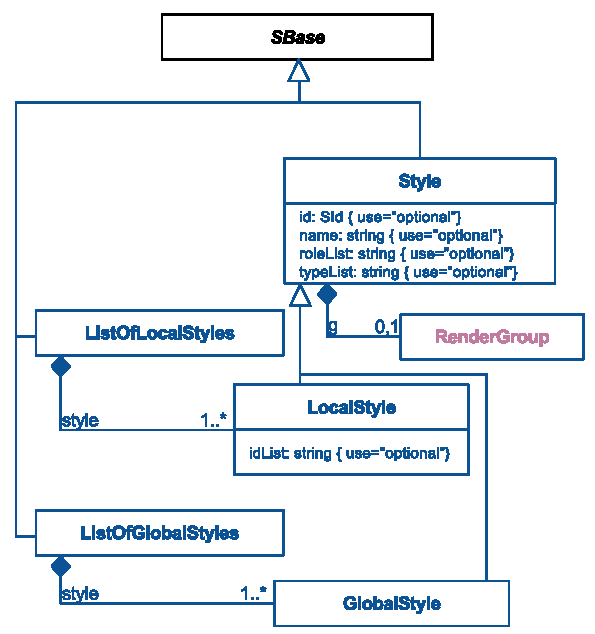
\includegraphics[width=\textwidth]{images/render-style-uml}\\
  \caption{A UML representation of the \Style object for the \RenderPackage.  See \ref{conventions} for conventions related to this figure. }
  \label{fig:style_render_uml}
\end{figure}
% ---------------------------------------------------------
\subsubsection{The \class{Style} class}
\label{style-class}

\Style is an abstract class that holds all the information that is common to both local and global styles (\ref{fig:style_render_uml}). The \Style object derives from the \SBase class and thus inherits any
attributes and elements that are present on this class.
A \Style element may contain exactly one \RenderGroup element.
In addition the \Style object has the optional attributes \token{id}, \token{name}, \token{roleList} and \token{typeList}.

The \RenderGroup element, \val{g}, is used to specify how the elements covered by this \Style object are to be rendered and is discussed fully in \ref{rendergroup-class}. 

\paragraph{The \fixttspace\token{id} attribute}

A \Style has an optional attribute \token{id} of type \primtype{SId} which can be used to uniquely identify this \Style object.

\paragraph{The \fixttspace\token{name} attribute}

A \Style has an optional attribute \token{name} of type
\primtype{string} which can be used to provide a more user friendly identifier.

\paragraph{The \fixttspace\token{roleList} attribute}

A \Style has an optional attribute \token{roleList} of type
\primtype{string}. The string value of the \token{roleList} attribute lists all the roles to which this \Style should be applied.

This attribute can be  used in conjunction with the \token{objectRole} attribute that is used to extend the \GraphicalObject class from the \LayoutPackage. If the string given as an \token{objectRole} value appears in the \token{roleList} attribute of some render information object, then that render information object
applies to the graphical object as shown in the snippet below. Note this relationship is only valid if there is no render information object that is more specific. \need{clarify this}

{\footnotesize
\begin{example}
<layout:layout>
   <layout:listOfGraphicalObjects>
      <layout:graphicalObject layout:id="go1" render:objectRole="Parameter">
         ...
      </layout:graphicalObject>
   </layout:listOfGraphicalObjects>
   <render:listOfLocalRenderInformation>
      <render:renderInformation render:id="FancyRenderer_GlobalDefault">
             ...
        <render:listOfStyles>
             <render:style render:id="style_1" render:roleList="Parameter">
                <g> ... </g>
             </render:style> 
        </render:listOfStyles>
      </render:renderInformation>
   </render:listOfGlobalRenderInformation>
</layout:listOfLayouts>
\end{example}
}

\TODO{check xml for layout is valid}


\paragraph{The \fixttspace\token{typeList} attribute}

A \Style has an optional attribute \token{typeList} of type
\StyleType. The string value of the \token{typeList} attributes contains one or more of the values from the \StyleType enumeration. The example snippet shows a particular style that is to be applied to both \class{SpeciesGlyph} and \class{SpeciesReferenceGlyph} objects from the \LayoutPackage.

{\footnotesize
\begin{example}
<layout:listOfLayouts>
   <render:listOfGlobalRenderInformation>
      <render:renderInformation render:id="FancyRenderer_GlobalDefault">
             ...
        <render:listOfStyles>
             <render:style render:id="style_1" render:typeList="SPECIESGLYPH SPECIESREFERENCEGLYPH">
                <g> ... </g>
             </render:style> 
        </render:listOfStyles>
      </render:renderInformation>
   </render:listOfGlobalRenderInformation>
</layout:listOfLayouts>
\end{example}
}

% ---------------------------------------------------------
\subsubsection{The \class{GlobalStyle} class}
\label{globalstyle-class}

The \GlobalStyle object derives from the \Style class and thus inherits
any attributes and elements that are present on this class. The \GlobalStyle class is used for objects in the \ListOfStyles element of a \GlobalRenderInformation object.



% ---------------------------------------------------------
\subsubsection{The \class{LocalStyle} class}
\label{localstyle-class}

The \LocalStyle object derives from the \Style class and thus inherits
any attributes and elements that are present on this class. It is identical to the \GlobalStyle object but has an additional optional \token{idList} attribute.

The \LocalStyle class is used for objects in the \ListOfStyles element of a \LocalRenderInformation object.

\paragraph{The \fixttspace\token{idList} attribute}

A \LocalStyle has an optional attribute \token{idList} of type
\primtype{string} which is a list of ids of layout objects to which this \Style should be applied. \need{are they space seperated ??}


% ---------------------------------------------------------
%----------------------------------------------------------
\subsection{Colors and Gradients}

All \RenderInformation objects may contain a \ListOfColorDefinitions containing objects of type \ColorDefinition and a \ListOfGradientDefinitions containing objects of type \GradientBase. Gradients consist of continuously smooth color transitions along a vector from one color to another, possibly followed by additional transitions along the same vector to other colors. Here the \RenderPackage borrows heavily from the SVG specification. These are described in more detail in this section. 
 
\subsubsection{The \class{ColorDefinition} class}
\label{colordefinition-class}

\begin{figure}[h!]
  \centering
  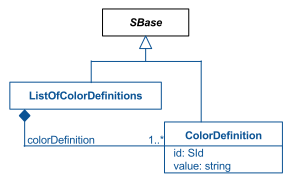
\includegraphics[width=\textwidth]{images/render-color-definition-uml}\\
  \caption{A UML representation of the \ColorDefinition object for the \RenderPackage.  See \ref{conventions} for conventions related to this figure. }
  \label{fig:color_render_uml}
\end{figure}


The \ColorDefinition object derives from the \SBase class and thus
inherits any attributes and elements that are present on this class.
In addition the \ColorDefinition object has the optional attributes \token{id} and \token{value}.

\paragraph{The \fixttspace\token{id} attribute}

A \ColorDefinition has an optional attribute \token{id} of type
\primtype{SId} which is used to give the \ColorDefinition an unique identifier within the /RenderInformation object.

\paragraph{The \fixttspace\token{value} attribute}

A \ColorDefinition has an optional attribute \token{value} of type
\primtype{string}. Color values are specified as a 6 to 8 digit hex string which defines the RGBA 
value of the color. If only the first six digits for the RGB value are given, 
the alpha value \need{what is alpha value} is assumed to be 0xFF which means that the color is totally 
opaque. Instead of specifying a color value, the value \val{none} can be given which is equivalent to 
no drawing at all.

\TODO{explain example - which has 6 digits and a \#}

{\footnotesize
\begin{example}
<listOfColorDefinitions>
  <colorDefinition id="darkred" value="#200000" />
       ...
</listOfColorDefinitions>
\end{example}
}


% ---------------------------------------------------------
\subsubsection{The \class{GradientBase} class}
\label{gradientbase-class}

\begin{figure}[h!]
  \centering
  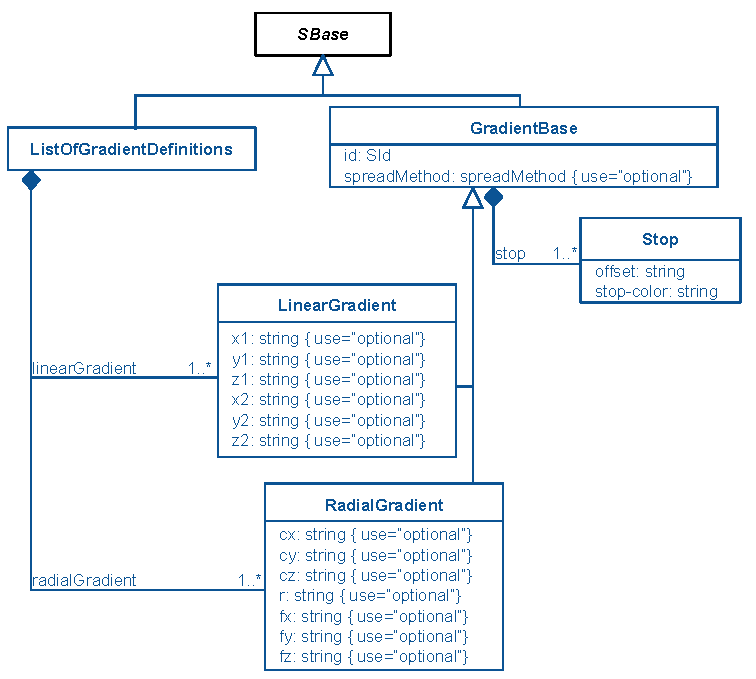
\includegraphics[width=\textwidth]{images/render-gradient-definitions-uml}\\
  \caption{A UML representation of the gradient objects for the \RenderPackage.  See \ref{conventions} for conventions related to this figure. }
  \label{fig:gradient_render_uml}
\end{figure}


\GradientBase is an abstract class that holds all the information that is common to both \RadialGradient and \LinearGradient objects (\ref{fig:style_render_uml}).The \GradientBase object derives from the \SBase class and thus inherits
any attributes and elements that are present on this class.
A \GradientBase may contain one \ListOfGradientStops element.
In addition the \GradientBase object has a required \token{id} attribute and an optional \token{spreadMethod} attribute.

\paragraph{The \fixttspace\token{id} attribute}

A \GradientBase has a required attribute \token{id} of type
\primtype{SId} which is used to uniquely identify or refernce a gradient within an \RenderInformation object.

\paragraph{The \fixttspace\token{spreadMethod} attribute}

A \GradientBase has an optional attribute \token{spreadMethod} of type
\GradientSpreadMethod that specifies the method that is
used to continue the gradient pattern if the vector points do not span the whole
bounding box of the object to which the gradient is applied. 

% ---------------------------------------------------------
\paragraph{The \class{ListOfGradientStops} class}
\label{listofgradientstops-class}

The \ListOfGradientStops object derives from the \class{ListOf} and
inherits the core attributes and subobjects from the \class{SBase}
class. It contains one or more objects of type \GradientStop.

\TODO{is this really a class - the uml suggests not but the deviser code has a listOf}

% ---------------------------------------------------------
\subsubsection{The \class{GradientStop} class}
\label{gradientstop-class}

As the name suggests the \GradientStop object is used to define "gradient stops" which are used in line with the SVG specification.
The \GradientStop object derives from the \SBase class and thus inherits
any attributes and elements that are present on this class.
In addition the \GradientStop object has the required attributes \token{offset} and \token{stop-color}.

\paragraph{The \fixttspace\token{offset} attribute}

A \GradientStop has a required attribute \token{offset} of type
\RelAbsVector which represents the relative distance from the starting point of the
gradient. Depending on the type of gradient, this is either the point defined by the
\token{x1},\token{y1} and \token{z1} attributes (\LinearGradient) or the \token{fx},
\token{fy} and \token{fz} attributes (\RadialGradient). This value is given as a positive percentage value.

\paragraph{The \fixttspace\token{stop-color} attribute}

A \GradientStop has a required attribute \token{stop-color} of type
\primtype{string} which defines the color for the given gradient stop. The
attributes value can either be given as a hexadecimal color value or as the id
of a \ColorDefinition object from the \ListOfColorDefinitions unless that \ColorDefinition specifies \val{none}. 
To specify the id of another gradient as the value of a \token{stop-color} attribute is 
considered an error.
In case the two points that define the gradient vector are identical, the area
is to be painted with a single color taken from the last gradient stop element.

There are a few rules that need to be considered when working with gradient stops.
Basically these rules are the same as defined by the SVG specification.

\begin{enumerate}
\item{The offset value of a gradient stop should be between 0\% and 100\%. If the offset lies outside of this value, the value is adjusted to be either 0\% is the given value is smaller than 0\% or to 100\% if the value is greater than 100\%.}
\item{The absolute part in any offset value is ignored, meaning it is considered to be 0.0 even if specified otherwise in a gradient stop.}
\item{The offset of any gradient stop has to be greater or equal to the offset of the preceding gradient stop. If a gradient stop has an offset that is smaller than the offset of the preceding stop, the offset is considered to have the same value as the offset of the preceding stop.}
\item{If two gradient stops have the same offset value, the last gradient stop with this offset value determines the color at this point in the gradient.}
\end{enumerate}
% ---------------------------------------------------------
\subsubsection{The \class{LinearGradient} class}
\label{lineargradient-class}

The \LinearGradient provides the vector points that define the start and end points to which the \GradientStop elements should be mapped.

The \LinearGradient object derives from the \GradientBase class and thus
inherits any attributes and elements that are present on this class.
In addition the \LinearGradient object has the attributes  \token{x1}, \token{y1},
\token{z1}, \token{x2}, \token{y2} and \token{z2}. As the names suggest these represent the x, y and z coordinates in a three dimensional Cartesian system. If only the x and y attributes are used a two dimensional viewport is assumed.

Since the value for the vector can be specified as an absolute value or one that is relative to the current viewport these attributes all have values of type \RelAbsVector.

\paragraph{The \fixttspace\token{x1}, \fixttspace\token{y1} and \fixttspace\token{z1} attributes}

The attributes \token{x1}, \token{y1} and token{z1} define the start point of the gradient in either two (\token{z1} undefined) or three dimensions.

\paragraph{The \fixttspace\token{x2}, \fixttspace\token{y2} and \fixttspace\token{z2} attributes}

The attributes \token{x2}, \token{y2} and token{z2} define the end point of the gradient in either two (\token{z2} undefined) or three dimensions.



\need{here we get into the issue that these are declared all optional with defaults!!}

{
  {\bf
Example of specifying the \LinearGradient shown in \ref{fig:lingrad}:
}
}
{\footnotesize
\begin{example}
<listOfGradientDefinitions>
  <linearGradient x1="12.5%" y1="25%" x2="87.5%" y2="75%">
    <stop offset="5%" stop-color="#000F60" />
    <stop offset="95%" stop-color="#000FF6" />
  </linearGradient>
        ...
</listOfGradientDefinitions>
\end{example}
}

\begin{figure}[h!]
  \centering
  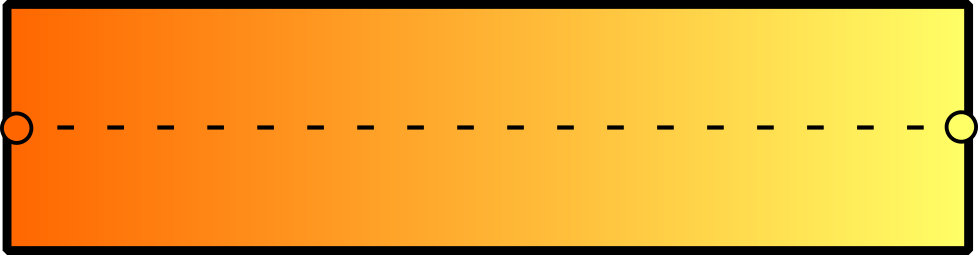
\includegraphics[scale=0.5]{figures/lingrad01.png}\\
  \caption{Example of a \LinearGradient}
  \label{fig:lingrad}
\end{figure}


% ---------------------------------------------------------
\subsubsection{The \class{RadialGradient} class}
\label{radialgradient-class}


The \RadialGradient object derives from the \GradientBase class and thus
inherits any attributes and elements that are present on this class.
In addition the \RadialGradient object has the seven attributes (each of type \RelAbsVector) that are used to define the center, radius and focal point of the gradient.



\paragraph{The \fixttspace\token{cx}, \fixttspace\token{cy} and \fixttspace\token{cz} attributes}

The attributes \token{cx}, \token{cy} and \token{cz} define the center of the gradient as a point in either two (\token{cz} undefined) or three dimensions.

\need{these have defaults!!}

\paragraph{The \fixttspace\token{r} attribute}

The attribute \token{r} defines the radius of the gradient and should be positive. If the radius is given in relative values, the relation is to the width as well as the height. This means that 
if the width of the bounding box and the height of the bounding box are not equal, \token{cx},\token{cy},\token{cz}
and \token{r} don't actually specify a circle, but an ellipse.

\paragraph{The \fixttspace\token{fx}, \fixttspace\token{fy} and \fixttspace\token{fz} attributes}

The attributes \token{fx}, \token{fy} and \token{fz} define the focal point of the gradient as a point in either two (\token{fz} undefined) or three dimensions. The gradient is drawn such that this point is mapped to the 0\% \GradientStop. If one of these attributes is left undeclared it is considered to be equal to the corresponding coordinate of the center point. If the focal point lies outside 
the circle, the focal point is considered to be located on the intersection of the the line from the center
point to the focal point and the sphere determined by the center point and the radius.


  {\bf
Example of specifying the \RadialGradient shown in \ref{fig:radgrad}:
}

{\footnotesize
\begin{example}
<listOfGradientDefinitions>
  <radialGradient cx="50%" cy="50%" r="300" fx="50%" fy="50%">
    <stop offset="0%" stop-color="#FF0000" />
    <stop offset="50%" stop-color="#0000FF" />
    <stop offset="100%" stop-color="#FF0000" />
  </radialGradient>
       ...
</listOfGradientDefinitions>
\end{example}
}

\begin{figure}[h!]
  \centering
  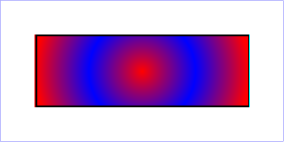
\includegraphics[scale=0.5]{figures/radgrad01.png}\\
  \caption{Example of a \RadialGradient}
  \label{fig:lingrad}
\end{figure}



%\begin{figure}[h!]
%  \centering
%  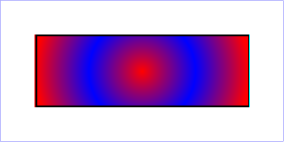
\includegraphics[scale=0.5]{figures/radgrad01.png}\\
%  \caption{Example of a \RadialGradient}
%  \label{fig:radgrad}
%\end{figure}



%--------------------------------------------------------
%---------------------------------------------------------
\subsection{Transformation}

In order to be able to display text that is not aligned horizontally or 
vertically or to effectively compose groups of objects from primitives, 
transformations like rotation, translation and scaling are needed. SVG, among 
other options, allows the user to specify a 3x3 matrix transformation matrix: 

\hspace*{0.4cm}
\begin{center}
\begin{math}\left[ \begin{array}{ccc} a & c & e \\ b & d & f \\ 0 & 0 & 1\end{array}\right]\end{math}
\end{center}
\hspace*{0.4cm}

Since the last row of the matrix is always 0 0 1, the matrix is specified as a 
six value vector. Therefore, in the render extension each group or graphical 
primitive is derived from the class \TransformationTwoD and can have a \token{transform} attribute just as in SVG.

\begin{figure}[h!]
  \centering
  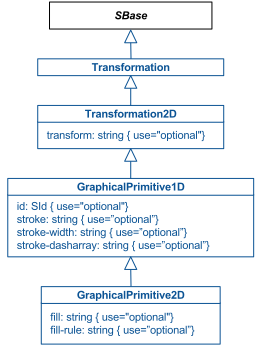
\includegraphics[scale=1.0]{images/render-base-classes-uml}\\
  \caption{A UML representation of the base graphical primitive classes for the \RenderPackage.  See \ref{conventions} for conventions related to this figure. }
  \label{fig:base_render_uml}
\end{figure}


% ---------------------------------------------------------
\subsubsection{The \class{Transformation} class}
\label{transformation-class}

The \Transformation class is a common base class for all elements that can be drawn.
Since both the \LayoutPackage and the \RenderPackage are currently limited to two dimensions, this class is only used as a base class for \TransformationTwoD and we leave the complete specification of this class for a future version of this document.


The \Transformation object derives from the \SBase class and thus
inherits any attributes and elements that are present on this class.
In addition the \Transformation object has the required \token{transform} attribute.

\paragraph{The \fixttspace\token{transform} attribute}

A \Transformation has a required attribute \token{transform} consisting
of an array of type \primtype{double}. This specifies an affine transformation matrix in three dimensions in which case the array must consist of exactly 12 values.

% ---------------------------------------------------------
\subsubsection{The \class{Transformation2D} class}
\label{transformationtwod-class}

Since the current render information specification only defines two dimensional objects, we derive a second class called \TransformationTwoD from \Transformation. As illustrated in \ref{fig:base_render_uml} the class \TransformationTwoD serves as the base class for all drawable 1D and 2D objects.

\paragraph{The \fixttspace\token{transform} attribute}

The \TransformationTwoD class restricts the transformation matrix to specify the six values of a 2D affine transformation. Thus the \token{transform} attribute consists of an array of exactly 6 values of type \primtype{double}. Thus the allowed 
value for the attribute has the form: \token{a, b, c, d, e, f}.

The values for \token{a},\token{b},\token{c},\token{d},\token{e} and \token{f} depend on the transformation operation components and the order in which those transformation components are executed.

There are four basic transformation operations that can be combined in a affine transformation matrix.  Details of these are given in Appendix \ref{apdx-transformations}.

All objects that are derived from \TransformationTwoD can have a transformation, this includes group elements. In contrast to other attributes on groups and children of groups, the transformation is not overwritten if it is specified in a child, but rather all transformations that are defined in an object hierarchy accumulate. Thus when a group specifies a transformation and a child of the group also sets a transformation, the transformation for the child has to be applied to the child only and the transformation that is set on the group has to be applied to the whole group, i.e. to all children of the group.

%--------------------------------------------------------
%--------------------------------------------------------
\subsection{GraphicalPrimitives}

The graphical primitives polygons, rectangles and ellipses are based on the 
corresponding elements from SVG. For lines, arcs and general path primitives, we 
introduce the \RenderCurve element which differs slightly from the \LayoutPackage \class{Curve}. 
Whereas \class{Point} objects in the \LayoutPackage could only contain 
absolute values for their coordinates, \RenderPoint objects in the \RenderPackage 
can contain relative coordinate values.  Two primitive abstract classes are defined to specify the common properties of 1D and 2D shapes.


% ---------------------------------------------------------
\subsubsection{The \class{GraphicalPrimitive1D} class}
\label{graphicalprimitiveoned-class}

The \GraphicalPrimitiveOneD object derives from the \TransformationTwoD
class and thus inherits any attributes and elements that are present on
this class (\ref{fig:base_render_uml}).
In addition the \GraphicalPrimitiveOneD object has the optional \token{id}, \token{stroke}, \token{stroke-width} and \token{stroke-dasharray} attributes.

\paragraph{The \fixttspace\token{id} attribute}

A \GraphicalPrimitiveOneD has an optional attribute \token{id} of type
\primtype{SId} which can be used to uniquely identify the object.

\paragraph{The \fixttspace\token{stroke} attribute}

A \GraphicalPrimitiveOneD has an optional attribute \token{stroke} of
type \primtype{string}. This is used to specify the color of the stroke that is used to draw the curve 
or the outline of geometric shapes. This \token{stroke}
attribute can either hold a color value or it can hold the id of a predefined
\ColorDefinition object.

\paragraph{The \fixttspace\token{stroke-width} attribute}

A \GraphicalPrimitiveOneD has an optional attribute \token{stroke-width}
of type \primtype{string} which specifies the width of the stroke to be used.

\paragraph{The \fixttspace\token{stroke-dasharray} attribute}

A \GraphicalPrimitiveOneD has an optional attribute
\token{stroke-dasharray} consisting of an array of values of type \primtype{unsigned
integer}. This list specifies the lengths of dashes and 
gaps that are used to draw the line. The individual numbers in the list are separated by commas. 
For example,  "5,10" would mean to draw 5 points, make a 10 point gap, draw 5 points etc. If the pattern is to start with a gap, the first number has to be 0.

It should be noted that if a style defines a stroke dasharray and this style is applied to a \class{Curve} from the \LayoutPackage, one has to watch out for the fact that the layout curves may contain breaks (if the end point of segment n is not identical to the starting point of segment n+1). In this case each of the unbroken line stretches is considered a separate curve object and the line stippling is applied to each curve. That means the line stippling is not continuously applied through the gap, but it starts again after the gap.


% ---------------------------------------------------------
\subsubsection{The \class{GraphicalPrimitive2D} class}
\label{graphicalprimitivetwod-class}

The \GraphicalPrimitiveTwoD object derives from the
\GraphicalPrimitiveOneD class and thus inherits any attributes and
elements that are present on this class (\ref{fig:base_render_uml}).
In addition the \GraphicalPrimitiveTwoD object has the optional \token{fill} and \token{fill-rule} attributes.

\paragraph{The \fixttspace\token{fill} attribute}

A \GraphicalPrimitiveTwoD has an optional attribute \token{fill} of type
\primtype{string} which specifies 
the fill style of the object. The fill style can either be a hexadecimal
color value, the id of a \ColorDefinition object or the id of a \GradientBase
object. 
Instead of a color or gradient id, \val{none} can be specified
 which means that the object is unfilled.


\paragraph{The \fixttspace\token{fill-rule} attribute}

A \GraphicalPrimitiveTwoD has an optional attribute \token{fill-rule} of
type \FillRule that can be used to specify how the shape should be filled. 

Currently the \token{fill-rule} attribute is only useful for polygons. No other shapes have alternating areas.

\need{might want to explain that a little more}
% ---------------------------------------------------------
\subsubsection{The \class{RenderCurve} class}
\label{rendercurve-class}
\begin{figure}[h!]
  \centering
  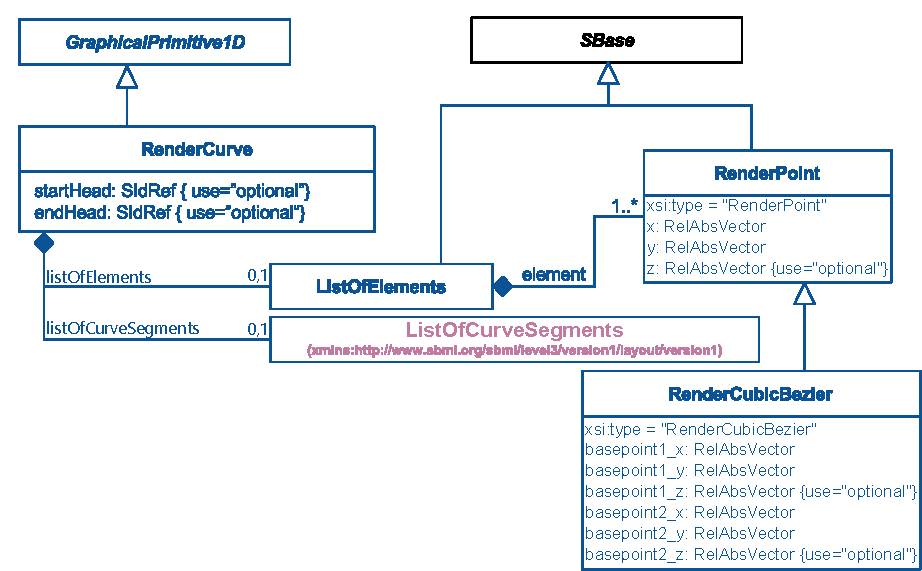
\includegraphics[width=\textwidth]{images/render-curve-uml}\\
  \caption{A UML representation of the \RenderCurve classes for the \RenderPackage.  See \ref{conventions} for conventions related to this figure. }
  \label{fig:curve_render_uml}
\end{figure}

Simple lines and complex curves are represented by a \RenderCurve element. 

The \RenderCurve object derives from the \GraphicalPrimitiveOneD class (see \ref{fig:curve_render_uml})
and thus inherits any attributes and elements that are present on this
class.
A \RenderCurve contains at most one \ListOfElements element.
In addition the \RenderCurve object has the optional attributes \token{startHead} and \token{endHead}.

\paragraph{The \fixttspace\token{startHead} attribute}

A \RenderCurve has an optional attribute \token{startHead} of type
\primtype{SIdRef} and points to the \LineEnding that should be applied to the start of the path.

\paragraph{The \fixttspace\token{endHead} attribute}

A \RenderCurve has an optional attribute \token{endHead} of type
\primtype{SIdRef} and points to the \LineEnding that should be applied to the end of the path.

% ---------------------------------------------------------
\paragraph{The \class{ListOfElements} class}
\label{listofelements-class}

The \ListOfElements object derives from the \class{ListOf} and inherits
the core attributes and subobjects from the \class{SBase} class. It
contains one or more objects of type \RenderPoint or of the derived type \RenderCubicBezier. The only restriction is that the first element must be a \RenderPoint.

\need{not sure how this fits into a curve - are you liertally specifying every point in the curve}

% ---------------------------------------------------------
\subsubsection{The \class{RenderPoint} class}
\label{renderpoint-class}

\RenderPoint objects are used to 
specify the individual curve segments.

The \RenderPoint object derives from the \SBase class and thus inherits
any attributes and elements that are present on this class.
In addition the \RenderPoint object has the required attributes \token{x} and \token{y} and the optional attribute \token{z}. It also has the required attribute \token{type} from the \val{xsi} namespaces.

\paragraph{The \fixttspace\token{x}, \fixttspace\token{y} and \fixttspace\token{z} attributes}

These three attributes are used to specify the coordinates of a  \RenderPoint in two (missing \token{z}) or three dimensions. They are of type \RelAbsVector and can thus specify a coordinate as either an absolute or relative value. The coordinate
values are always with respect to the bounding box of the layout object to which the
render information applies.

\paragraph{The \fixttspace\token{xsi:type} attribute}

For a \RenderPoint object this attribute will always have the value \val{RenderPoint}.


% ---------------------------------------------------------
\subsubsection{The \class{RenderCubicBezier} class}
\label{rendercubicbezier-class}


The \RenderCubicBezier object derives from the \RenderPoint class and
thus inherits any attributes and elements that are present on this
class.
In addition the \RenderCubicBezier object has the required attributes \token{basepoint1\_x}, \token{basepoint1\_y}, \token{basepoint2\_x} and \token{basepoint2\_y}. It also has the optional attributes \token{basepoint1\_z} and \token{basepoint2\_z}.

\paragraph{The \fixttspace\token{basepoint1\_x}, \fixttspace\token{basepoint1\_y} and \fixttspace\token{basepoint1\_z} attributes}

These three attributes are used to specify the coordinates of the first basepoint of a \RenderCubicBezier in two (missing \token{basepoint1\_z}) or three dimensions. They are of type \RelAbsVector and can thus specify a coordinate as either an absolute or relative value. The coordinate
values are always with respect to the bounding box of the layout object to which the
render information applies.


\paragraph{The \fixttspace\token{basepoint2\_x}, \fixttspace\token{basepoint2\_y} and \fixttspace\token{basepoint2\_z} attributes}

These three attributes are used to specify the coordinates of the second basepoint of a \RenderCubicBezier in two (missing \token{basepoint2\_z}) or three dimensions. They are of type \RelAbsVector and can thus specify a coordinate as either an absolute or relative value. The coordinate
values are always with respect to the bounding box of the layout object to which the
render information applies.

\paragraph{The \fixttspace\token{xsi:type} attribute}

For a \RenderCubicBezier object this attribute will always have the value \val{RenderCubicBezier}.



The example snippet illustrates the definition of a \RenderCurve that \need{fill in what it actually represents cos I'm not sure}

{\footnotesize
\begin{example}
 <g ...>
  <curve stroke-width="2.0" stroke="#000000" >
   <listOfElements>
     <element xsi:type="RenderPoint" x="0%" y="50%" />
     <element xsi:type="RenderPoint" x="100%" y="50%" />
     <element xsi:type="RenderCubicBezier" x="0%" y="50%"
              basepoint1\_x="50%" basepoint1\_y="90%"
              basepoint2\_x="50%" basepoint2\_y="90%" />
   </listOfElements>
  </curve>
    ...
</g> 
\end{example}
} 
%---------------------------------------------------------
%---------------------------------------------------------
\subsection{Geometric Shapes}
\label{shapes}

This section details the classes of geometric objects that can be defined using the transformations and graphical primitives described (see \ref{fig:group_render_uml}).

\begin{figure}[h!]
  \centering
  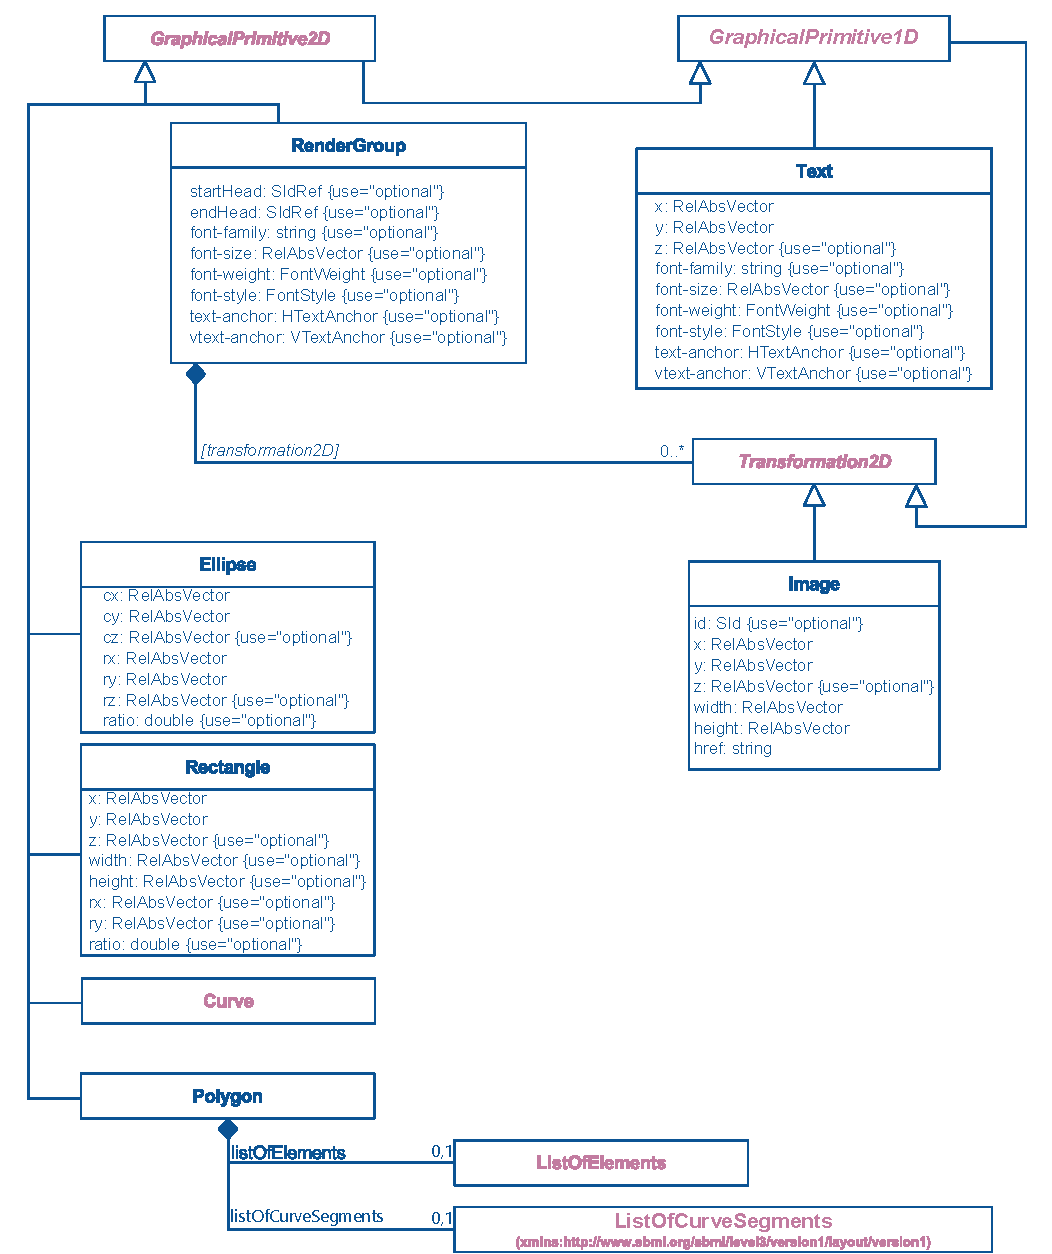
\includegraphics[width=\textwidth]{images/render-group-uml}\\
  \caption{A UML representation of the graphical primitive classes for the \RenderPackage.  See \ref{conventions} for conventions related to this figure. }
  \label{fig:group_render_uml}
\end{figure}


% ---------------------------------------------------------
\subsubsection{The \class{Polygon} class}
\label{polygon-class}

A \Polygon object is made up of a \texttt{polygon} element which contains a 
\ListOfElements that defines the edge of the polygon.

The major difference to the \RenderCurve 
object is that the individual curve segments can only be straight lines and the last point
 of the curve is connected to the first, so the polygon is always closed. 
Therefore, the polygon can have a fill style 
that determines how the inside of the polygon is to be rendered.

The example snippet shows the render specification of a \Polygon.

{\footnotesize
\begin{example}
<g ...>
  <polygon stroke="#000000" stroke-width="3" fill="#FF0000">
    <listOfElements>
      <element xsi:type="RenderPoint" x="100%" y="33%"/>
      <element xsi:type="RenderPoint" x="20%" y="100%"/>
      <element xsi:type="RenderPoint" x="50%" y="0"/>
      <element xsi:type="RenderPoint" x="80%" y="100%"/>
      <element xsi:type="RenderPoint" x="0" y="33%"/>
    </listOfElements>
  </polygon>
     ...
</g>

\end{example}
}

\need{it would be better if the xml snippet encoded the figure}

\begin{figure}[!ht]
\begin{center}
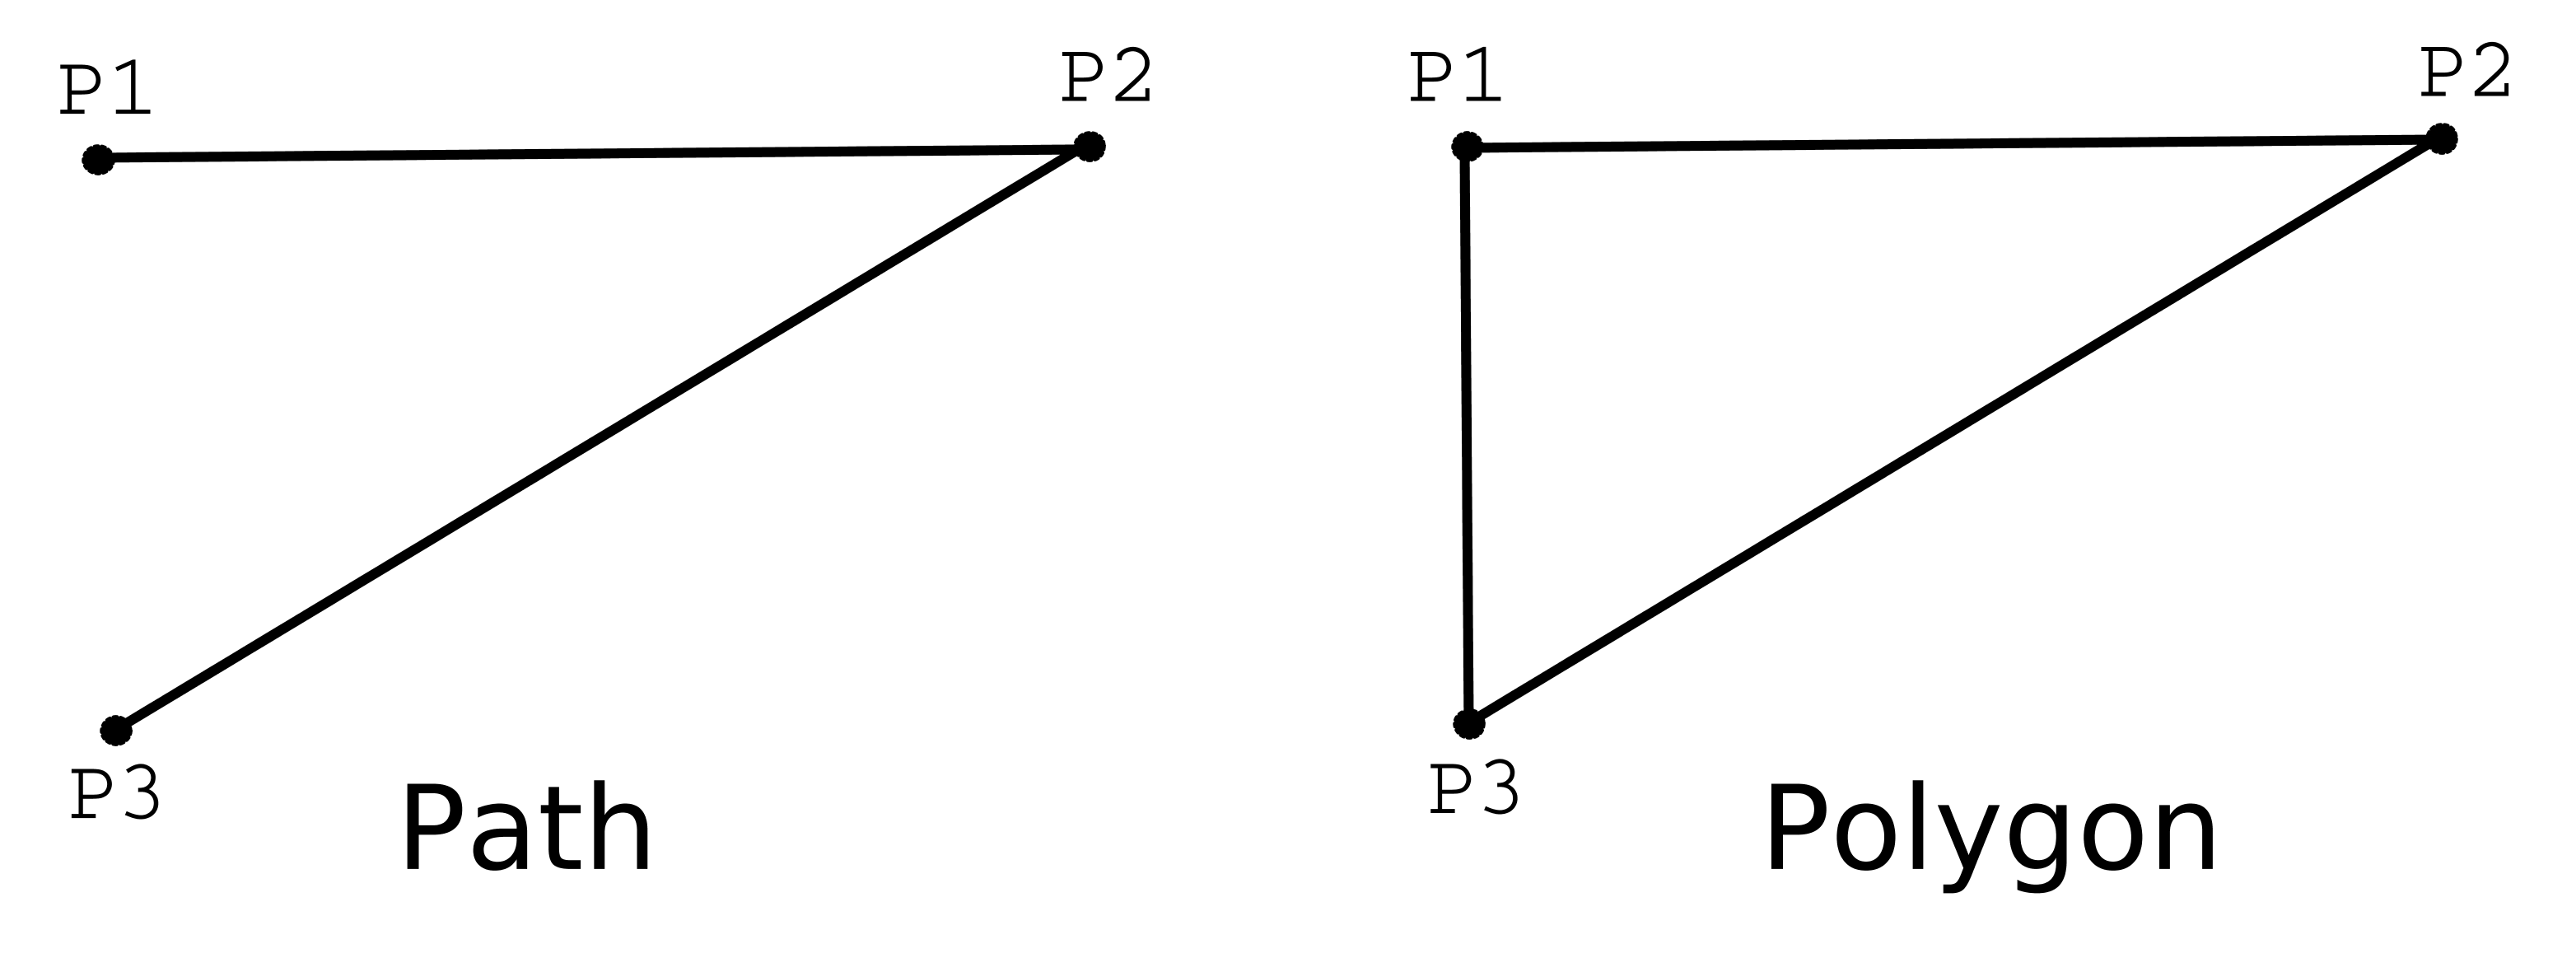
\includegraphics[scale=0.10]{figures/PathVsPolygon}
\end{center}
\caption{Rendering of a Path vs. rendering of a Polygon with the same base points}
\label{PathVsPolygon}
\end{figure}



% ---------------------------------------------------------
\subsubsection{The \class{Rectangle} class}
\label{renderrectangle-class}

The \RenderRectangle object was taken from the SVG specification and allows the definition of 
rectangles with or without rounded edges. 

The \RenderRectangle object derives from the \GraphicalPrimitiveTwoD
class and thus inherits any attributes and elements that are present on
this class.
In addition the \RenderRectangle object has the required attributes \token{x}, \token{y}, \token{height}, and \token{width} and the optional attributes \token{z}, \token{rx} and token{ry}.

\paragraph{The \fixttspace\token{x}, \fixttspace\token{y} and \fixttspace\token{z}  attributes}

These attributes are of type
\RelAbsVector and specify its position within the 
bounding box of the enclosing layout object.

\paragraph{The \fixttspace\token{width} and \fixttspace\token{height} attribute}

These attributes are of type
\RelAbsVector and specify the width and height of the rectangle, 
either in absolute values or as a percentage of the width and height of the 
enclosing bounding box. 

\paragraph{The \fixttspace\token{rx} and \fixttspace\token{ry} attributes}

These attributes are of type
\RelAbsVector and specify the radius of the corner curvature. If only \token{rx} or \token{ry} 
is specified, the other is presumed to have the same value as the one given. If no values are supplied this means that the edges are not rounded.
The relative values in rx and ry are in relation to the width and the height of the rectangle respectively.
So a value of $10\%$ for rx means the radius of the corner is $10\%$ of the width of the rectangle. 


% ---------------------------------------------------------
\subsubsection{The \class{Ellipse} class}
\label{renderellipse-class}


The \RenderEllipse object derives from the \GraphicalPrimitiveTwoD class
and thus inherits any attributes and elements that are present on this
class.
In addition the \RenderEllipse object has the required attributes \token{cx}, \token{cy} and \token{rx} and the optional attributes \token{cz} and \token{ry}.

\paragraph{The \fixttspace\token{cx}, \fixttspace\token{cy} and \fixttspace\token{cz}  attributes}

These attributes are of type
\RelAbsVector and specify the centre of the ellipse.

\paragraph{The \fixttspace\token{rx} and \fixttspace\token{ry} attribute}

These attributes are of type
\RelAbsVector and specify the radius of the eillipse along the x-axis and y-axis respectively. If only one value is specified the other is assumed to have the same value. 

Circles are a special case where the \token{rx} and \token{ry} attributes have the same value.

% ---------------------------------------------------------
\subsubsection{The \class{Text} class}
\label{text-class}

In order to draw text, we use the \token{text} element from SVG with slight 
modifications. For reasons of simplicity, we limit the display of text to normal text, 
outlined or filled-outlined text are not supported.

Since we have a right handed coordinate system, the positive y axis normally faces downward on the screen if the positive
z-axis goes into the screen. This means that text actually has to be renderer with the top towards lower y-values.


The \Text object derives from the \GraphicalPrimitiveOneD class and thus
inherits any attributes and elements that are present on this class.
In addition the \Text object has the required attributes \token{x} and \token{y} and the optional attributes \token{z}, \token{font-size}, \token{font-family}, \token{font-weight}, \token{font-style}, \token{text-anchor} and \token{vtext-anchor}.

\paragraph{The \fixttspace\token{x} attribute}

The \token{x} attribute is of type
\RelAbsVector and specifies the position of the horizontal text anchor.

\paragraph{The \fixttspace\token{y} attribute}

The \token{y} attribute is of type
\RelAbsVector and specifies the position of the vertical text anchor.

\paragraph{The \fixttspace\token{z} attribute}

The \token{z} attribute is of type
\RelAbsVector and directly specifies the depth value of the text element since there is no alignment attribute for text in the third dimension.

\paragraph{The \fixttspace\token{font-size} attribute}

A \Text has an optional attribute \token{font-size} of type \RelAbsVector which must have a positive value. In the case of a relative value it specifies a percentage of the
height of the corresponding object. Combinations of relative and absolute values are not allowed.


\paragraph{The \fixttspace\token{font-family} attribute}

A \Text has an optional attribute \token{font-family} of type
\FontFamily.  This limits the 
choice of the \token{font-family} attribute to the generic families \val{serif}, \val{sans-serif}
and \val{monospace}. However, since those only apply to western languages, it can make
sense to use other values for \token{font-family} in certain cases.

\paragraph{The \fixttspace\token{font-weight} attribute}

A \Text has an optional attribute \token{font-weight} of type
\FontWeight and specifies if the text is to be \val{normal} or \val{bold}.

\paragraph{The \fixttspace\token{font-style} attribute}

A \Text has an optional attribute \token{font-style} of type \FontStyle which specifies whether the style for the text is to be \val{italic} or \val{normal}.

\paragraph{The \fixttspace\token{text-anchor} attribute}

A \Text has an optional attribute \token{text-anchor} of type
\HTextAnchor which specifies the horizontal alignment of the text (see \ref{apdx-text-anchor}).

\paragraph{The \fixttspace\token{vtext-anchor} attribute}

A \Text has an optional attribute \token{vtext-anchor} of type
\VTextAnchor which specifes the vertical alignment of the text (see \ref{apdx-text-anchor}).

Note that since the way text is drawn is completely determined by the font specification, text elements should ignore the stroke-width attribute that they inherit from \GraphicalPrimitiveOneD.

% ---------------------------------------------------------
\subsubsection{The \class{Image} class}
\label{image-class}

To include bitmaps into a graphical representation we use the \Image element 
from SVG. However the use of the \Image element to include complete SVG 
vector images has been excluded.


The \Image object derives from the \TransformationTwoD class and thus
inherits any attributes and elements that are present on this class.
In addition the \Image object has the optional attributes \token{id} and \token{z} and the attributes \token{x}, \token{y}, \token{width}, \token{height} and \token{href} that are required..

\paragraph{The \fixttspace\token{id} attribute}

An \Image has an optional attribute \token{id} of type \primtype{SId} that can be used to give the \Image a unique identifier.

\paragraph{The \fixttspace\token{x}, \fixttspace\token{y} and \fixttspace\token{z}  attributes}

These attributes are of type
\RelAbsVector and specify the position of the \Image within it's bounding box.

\paragraph{The \fixttspace\token{width} and \token{height} attributes}

These attributes are of type
\RelAbsVector and specify the width and height to be used for the \Image. Thes atrributes are both required.

\paragraph{The \fixttspace\token{href} attribute}

An \Image has a required attribute \token{href} of type
\primtype{string} which encodes a reference to an external JPEG or PNG file. The reference must be an absolute or relative path to a local file.
Non-local image resources (e.g. from the net) are currently not supported.


Note that if the referenced image is larger then the given 
width and height, it has to be scaled to the given dimensions.
If the referenced resource can not be found, it is up to the application if nothing is drawn or some place holder is displayed.
Preferably the user would get some kind of notification about the missing resource.

The example shows the encoding for including the file Glucose.png.
{
\footnotesize
\begin{example}
 <g ...>
  <image x="10%" y="10%" width="80" height="100" href="Glucose.png" /> 
      ...
</g> 
\end{example}
}


% ---------------------------------------------------------
\subsubsection{The \class{RenderGroup} class}
\label{rendergroup-class}

Similar to the technique used by SVG, several graphical primitives can be grouped inside a \texttt{g} 
element to generate more complex render information.



The \RenderGroup object derives from the \GraphicalPrimitiveTwoD class
and thus inherits any attributes and elements that are present on this
class.
A \RenderGroup contains exactly one \ListOfElements element.
In addition the \RenderGroup object has the following attributes.

\paragraph{The \fixttspace\token{startHead} and \fixttspace\token{endHead} attributes}

A \RenderGroup has optional attributes \token{startHead} and \token{endHead} of type
\primtype{SIdRef} which point to a \LineEnding for the start and end of curves respectively. These attributes only apply to \RenderCurve objects from the layout, not
to \RenderCurve objects within the group/need{is that not a contradiction}. Since those two attributes only make sense on the outermost group of a style,
they are to be ignored on all other groups. 

\paragraph{The \fixttspace\token{font-size}, \fixttspace\token{font-family}, \fixttspace\token{font-weight} , \fixttspace\token{font-style},  \fixttspace\token{text-anchor} and\fixttspace\token{vtext-anchor} attributes}

These attributes are of the same types as the identically named attributes specified on the \Text object.   If any of those attributes is specified for a \RenderGroup object, it 
specifies the corresponding attribute for all graphical primitives and groups 
defined within this group. If a graphical primitive or a group redefines one or 
more of those attributes, the newly defined values take effect.

\need{here we have a whole bath of default values}
%---------------------------------------------------------
% ---------------------------------------------------------
\subsection{The \class{LineEnding} class}
\label{lineending-class}

In many graphs the relations between nodes are depicted by lines and often the 
type of relation is encoded in the line ending. For this reason, the render
extension provides ways to specify a set of arbitrary line endings and means to
apply those to other objects. Appendix C provides more information (\ref{mapping}).

\begin{figure}[h!]
  \centering
  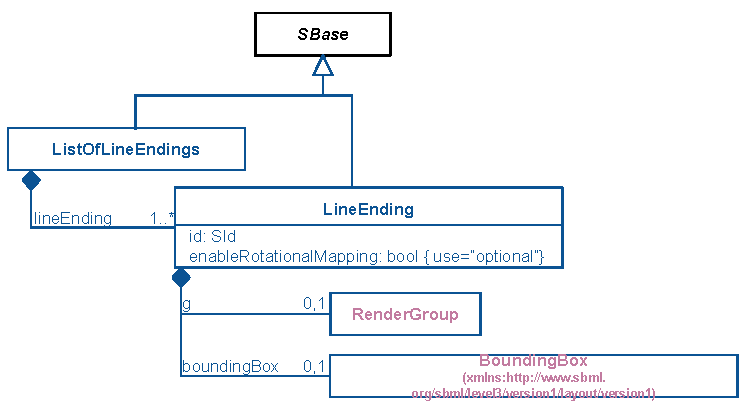
\includegraphics[width=\textwidth]{images/render-line-endings-uml}\\
  \caption{A UML representation of the \LineEnding class for the \RenderPackage.  See \ref{conventions} for conventions related to this figure. }
  \label{fig:line_ending_render_uml}
\end{figure}


The \LineEnding object derives from the \GraphicalPrimitiveTwoD class
and thus inherits any attributes and elements that are present on this
class.
A \LineEnding contains exactly one \class{BoundingBox} element from the \LayoutPackage which allows the \token{position} and \token{dimensions} to be specified. It also contains a \RenderGroup element which provides the necessarty render information for the line ending.
  
In addition the \LineEnding object has the a required \token{id} attribute and an optional \token{enableRotationalMapping} attribute.

\paragraph{The \fixttspace\token{id} attribute}

A \LineEnding has a required attribute \token{id} of type
\primtype{SId} which allows a unique identifer to be provided for this \LineEnding so that it may be referenced by other objects. The \token{startHead} and \token{endHead} attributes on a \RenderCurve expect to point to the \token{id} of a \LineEnding.

\paragraph{The \fixttspace\token{enableRotationalMapping} attribute}

A \LineEnding has an optional attribute \token{enableRotationalMapping}
of type \primtype{boolean} which specifies whether a line ending
will be rotated depending on the slope of the line it is applied to (if \val{true}) or if it is
drawn just the way it was specified (if \val{false}).
\begin{figure}[h!]
\begin{center}
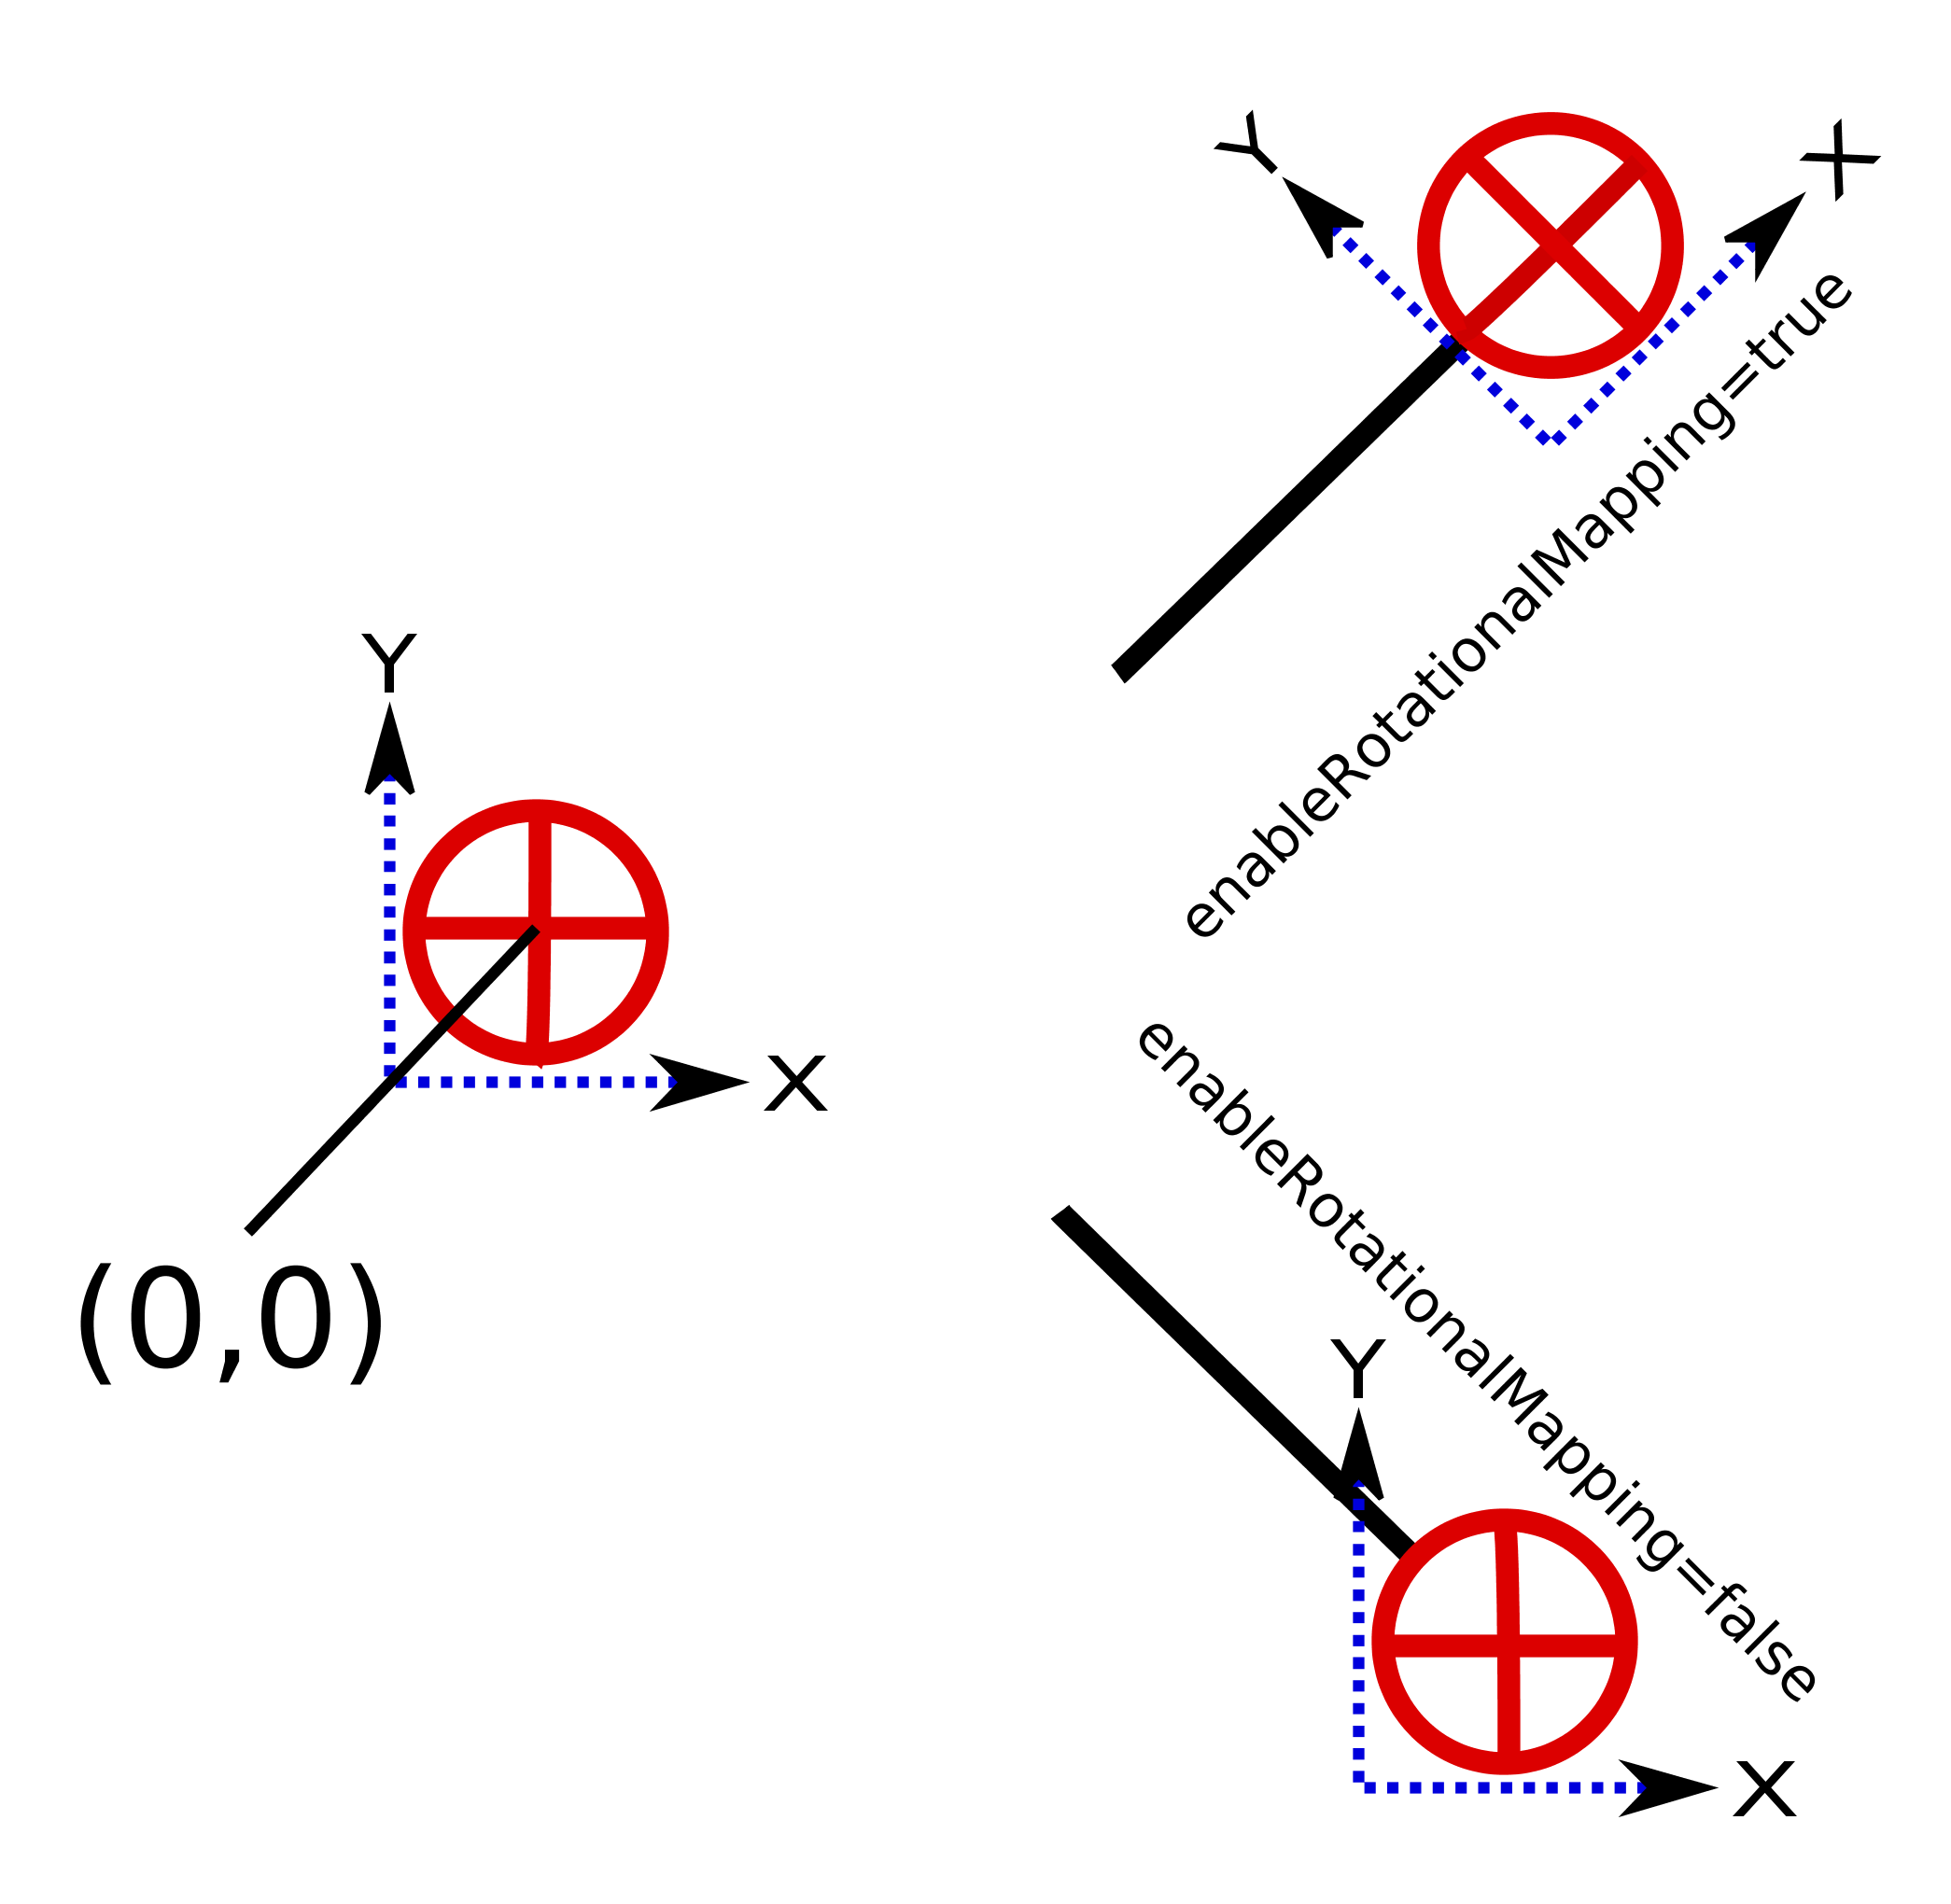
\includegraphics[scale=0.15]{figures/EnableRotationalMapping.png}
\end{center}
\caption{example of a line ending with and without rotation mapping enabled}
\label{EnableRotationalMapping}
\end{figure}

It should be noted that the top level \RenderGroup in a \LineEnding differs from top level groups in normal graphical elements in one respect. The top level \RenderGroup of a \LineEnding inherits all attributes from the line it is applied to save for the attributes for the line endings themselves. This way a style sheet can define one line ending which can be applied to lines of different colors and it inherits the color from the line.
If the group also inherited the attributes for the line endings and it contained a \texttt{curve} element itself, we would have generated an endless loop.

The example snippet shows the definition of an arrow head.

{
\footnotesize
\begin{example}
<lineEnding id="SimpleArrowHead">
 <boundingBox>
   <position x="-10.0" y="-4.0" />
   <dimensions width="12.0" height="8.0"/>
 </boundingBox>
 <g>
   <polygon>
     <curve>
       <listOfCurveSegments>
         <curveSegment xsi:type="LineSegment">
           <start x="100%" y="50%" />
           <end x="0%" y="100%" />
         </curveSegment>
         <curveSegment xsi:type="LineSegment">
           <start x="0%" y="100%" />
           <end x="0%" y="0%" />
         </curveSegment>
       </listOfCurveSegments>
     </curve>
   </polygon>
 </g>
</lineEnding>  
\end{example}
}


